%!TEX root = ../MasterThesis.tex

\section{System Design Proposal}
\label{sec:design_proposal}

As the previous section explained in detail, existing architectural approaches are of limited use for the design of a collaborative system to support the \gls{E-commerce} fraud investigation scenario described in Section~\ref{sec:scope_thesis}. The leading approach for such a system will have to combine the best characteristics from the Web Service and the Semantic Web designs. \\

As for the Web Service approach, the most valuable aspects of it are: \@

\begin{itemize}
	\item access to the \gls{HTTP} endpoint can be limited to a certain set of communication partners
	\item these partners have to authenticate with the Web Service first
	\item based on the identification of the partners only certain parts of information can be returned, and execution of operations can be restricted
\end{itemize}

Looking at the Semantic Web approach, it's most interesting functionalities are: \@

\begin{itemize}
	\item providing information in a semantically self-contained way
	\item the ability to merge information from different \gls{RDF} data stores
	\item the graph-based data model of \gls{RDF}
	\item the usage of \gls{SPARQL} to query and analyze the combined data set
\end{itemize}

In the following section the thesis will come up with an approach that uses the fundamental technologies from the Semantic Web for information sharing and integration as well as Peer-to-Peer communication technologies for securing and restricting access to the \gls{RDF} data sets from the relevant participants of the \gls{E-commerce} fraud investigation scenario. It will start with a discussion of the semantics of the underlying \gls{RDF} files and how these can be combined across various organizations. After that it shows how these information can be provided to the relevant parties in the investigation scenario. It will continue with a detailed look into the \gls{P2P} architectures that can be used for the proposed solution and will close with a conclusion about the solution that has been worked out.

\subsection{Vocabulary alignment}
\label{subsec:vocab_align}

Although the \gls{RDF} format has build-in support for merging information from different data sources, this functionality is only working as expected if the ``triples'' in the data sources are using the same \gls{URI}s to refer to the same subjects or objects. In that case merging the ``triples'' from different \gls{RDF} data files will result in a graph holding the combined information as shown in Figure~\ref{fig:images_combine_rdf_graph}.\@

\begin{figure}[H]
	\centering
		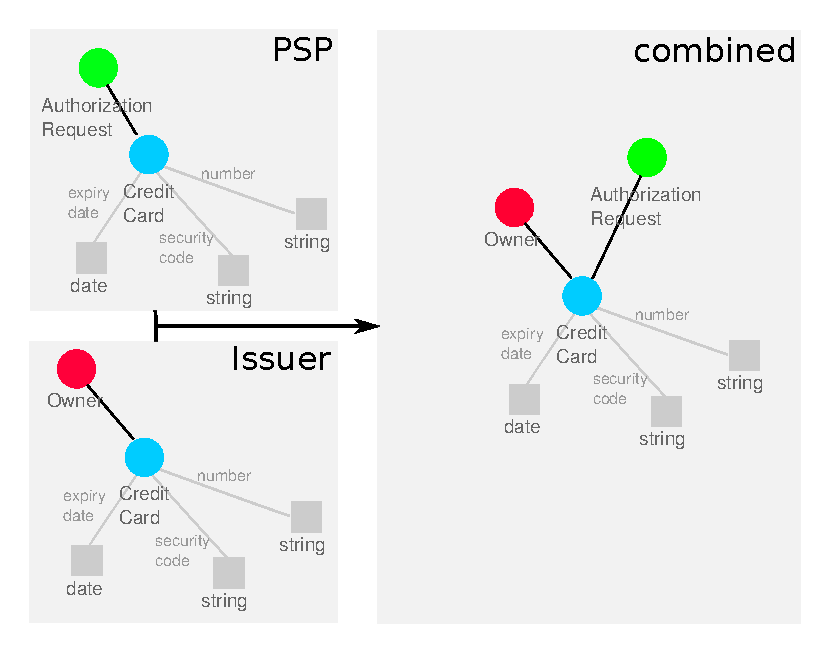
\includegraphics[width=0.9\columnwidth]{images/combine_rdf_graph.pdf}
	\caption{Combining two \gls{RDF} files containing the same credit card entity}
\label{fig:images_combine_rdf_graph}
\end{figure}

As a major objective of the \gls{E-commerce} fraud investigation system is to bring the various transactional information from online merchants, \gls{PSP} and issuers together, combine them and analyze the resulting graph from different viewpoints, the information exchanged between the relevant participants have to follow a common schema. A possible approach is to define a completely new schema for the proposed system and share it with every possible stakeholder. This schema will define the entities and relations specific to the \gls{E-commerce} fraud investigation process and would be expressed in \gls{RDFS} format. A major drawback of this approach is, that new partners of the system will have to do the conversion of their internal data structures to an \gls{RDF} file, that is compatible with the specific schema definition, before being able to participate in it. \\

Therefore a better approach is to take a look into commonly used \gls{RDF} schemata and vocabularies, and try to figure out if they can be used for describing the information, that need to be exchanged between participants of the \gls{E-commerce} fraud investigation system. When consulting the Semantic Web community for commonly agreed upon and highly referenced \gls{RDF} schema definitions, one will come up with this list (see Table~\ref{tab:used_vocab_rdf}):\@

\begin{table}[H]
\centering
\begin{tabular}{p{3cm}llp{4.5cm}}
\hline
\textbf{Name} & \textbf{Prefix} & \textbf{Describes} & \textbf{Namespace URI} \\
\hline
Dublin Core & dc: & Meta data & \url{http://purl.org/dc/terms/} \\
\hline
FOAF & foaf: & People & \url{http://xmlns.com/foaf/0.1/} \\
\hline
Geo & pos: & Positions & \url{http://www.w3.org/2003/01/geo/wgs84\_pos\#} \\
\hline
Geo Names & gn: & Locations & \url{http://www.geonames.org/ontology\#} \\
\hline
Good Relations & gr: & Products & \url{http://purl.org/goodrelations/v1\#} \\
\hline
RDF & rdf: & Core framework & \url{http://www.w3.org/1999/02/22-rdf-syntax-ns\#} \\
\hline
RDFS & rdfs: & RDF vocabularies & \url{http://www.w3.org/2000/01/rdf-schema\#} \\
\hline
Schema.org & schema: & Schema.org vocabularies & \url{http://schema.org/} \\
\hline
SKOS & skos: & Controlled vocabularies & \url{http://www.w3.org/2004/02/skos/core\#} \\
\hline
vCard & vcard: & Business Cards & \url{http://www.w3.org/2006/vcard/ns\#} \\
\hline
Web Ontology Language & owl: & Ontologies & \url{http://www.w3.org/2002/07/owl\#} \\
\hline
XML Schema Datatypes & xsd: & Data types & \url{http://www.w3.org/2001/XMLSchema\#} \\
\hline
\end{tabular}
\caption[Commonly used \gls{RDF} vocabularies on the Web]{Commonly used \gls{RDF} vocabularies on the Web \citep[pg. 41]{wood2014linked}}
\label{tab:used_vocab_rdf}
\end{table}

Based on these schema specifications describing a fictive consumer named ``Max Mustermann'' incl.\ his home address can be done by combining data from the \gls{FOAF} and \gls{vCard} namespaces in an \gls{RDF} file, such as described in Listing~\ref{lst:sample_customer_mustermann} and visualized as graph in Figure~\ref{fig:images_sample_customer}. \@

\begin{listing}[H]
  \inputminted[linenos,
               numbersep=5pt,
               breaklines=true,
               frame=lines]{TURTLE}
               {./samples/sample_customer_mustermann.ttl}
  \caption{Personal related information about a fictive consumer in \gls{RDF}}
\label{lst:sample_customer_mustermann}
\end{listing}

\begin{figure}[H]
	\centering
		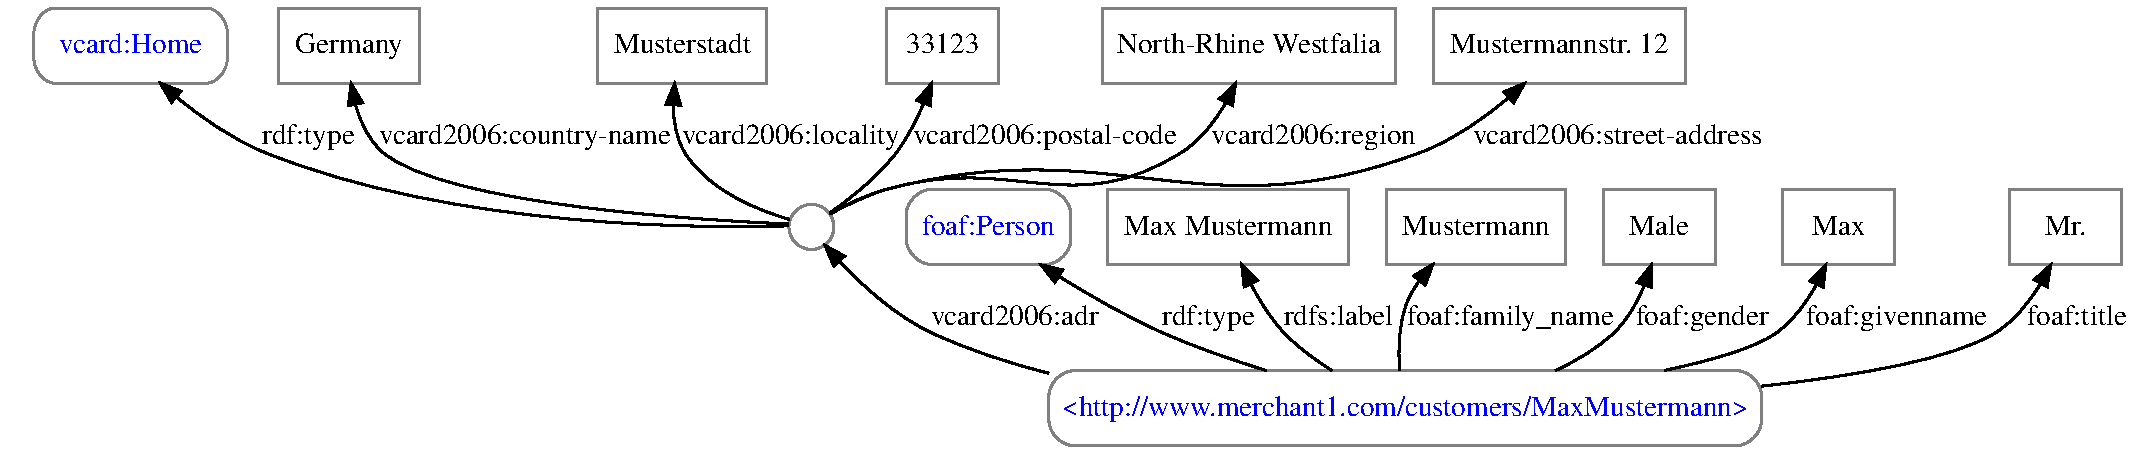
\includegraphics[width=\columnwidth]{images/sample_customer_mustermann.pdf}
	\caption{Graph representation of consumer information from Listing~\ref{lst:sample_customer_mustermann}}
\label{fig:images_sample_customer}
\end{figure}

Looking back to the initial data model from Section~\ref{sec:system_concept} one can map the information, that are currently available in the \gls{E-commerce} scenario, to the existing \gls{RDF} vocabularies such as follows (see Table~\ref{tab:map_tx_rdf_vocab}):\@

\begin{table}[H]
\centering
\begin{tabular}{p{5cm}l}
\hline
\textbf{Information} & \textbf{RDF vocabulary} \\
\hline
Consumer & FOAF \\
\hline
Credit Card Owner & FOAF \\
\hline
Billing Address & vCard \\
\hline
Shipping Address & vCard \\
\hline
Location Information & Geo Names \\
\hline
Merchant & GoodRelations \\
\hline
Items & GoodRelations \\
\hline
Item Categories & GoodRelations \\
\hline
Brands & GoodRelations \\
\hline
Payment Types & GoodRelations \\
\hline
\end{tabular}
\caption{Possible usage of \gls{RDF} vocabularies for \gls{E-commerce} transaction information}
\label{tab:map_tx_rdf_vocab}
\end{table}

As this table shows there are some parts of the \gls{E-commerce} data model that can be expressed with existing \gls{RDF} vocabularies extensively --- such as personal related information via \gls{FOAF} and \gls{vCard}, whereas other parts can not be stated in-depth (e.g. credit card information), or are not mentioned at all (e.g. tracking of the delivery). Additionally some of the vocabularies are no longer actively maintained, such as GoodRelations. Due to these circumstances one usually have to build an own ontology that fills in the missing pieces and refers to the existing concepts where appropriate. When modeling the information of a credit card as displayed in Figure~\ref{fig:images_data_model} one can come up with the \gls{RDFS} specification shown in Listing~\ref{lst:credit_card_vocab}. \@

\begin{listing}[H]
  \inputminted[linenos,
               numbersep=5pt,
               breaklines=true,
               frame=lines]{TURTLE}
               {./samples/vocab_credit_card.ttl}
  \caption{A specification for a credit card in \gls{RDFS}}
\label{lst:credit_card_vocab}
\end{listing}

As mentioned before building a new ontology for handling the \gls{E-commerce} fraud investigation process is not the best approach. The result would be that participants have to access, understand and implement the desired \gls{RDF} file format first, before they can share their information in the collaborative system. Looking back at the list of existing ontologies and vocabularies, that are actively used on the Web today, one will find the Schema.org vocabulary definition \citep{Schema.org}. This vocabulary was initially designed by the leading search engines to allow Web site authors to markup their \gls{HTML} documents in a way, that they are better understood by those search engines. It is actively maintained, includes new concepts with each release and also offers an extension mechanism to implement additional vocabularies that are not part of the core specification \citep{SchemaExtensions}. In one of the past releases of the Schema.org specification they also included all of the existing concepts of the GoodRelation ontology \citep{SchemaGoodRelation}. \\

As the merchants will provide semantic meta data for \gls{SEO} in the vocabulary of Schema.org already, one can re-use parts of these information for the \gls{E-commerce} fraud investigation. Also the wide-ranging aspects that Schema.org declares make it a good fit to the \gls{E-commerce} fraud investigation scenario. When mapping the initial data model from Section~\ref{sec:system_concept} to the Schema.org specifications one will come up with the following approach as displayed in Figure~\ref{fig:images_schema_org}. \@

\begin{figure}[H]
	\centering
		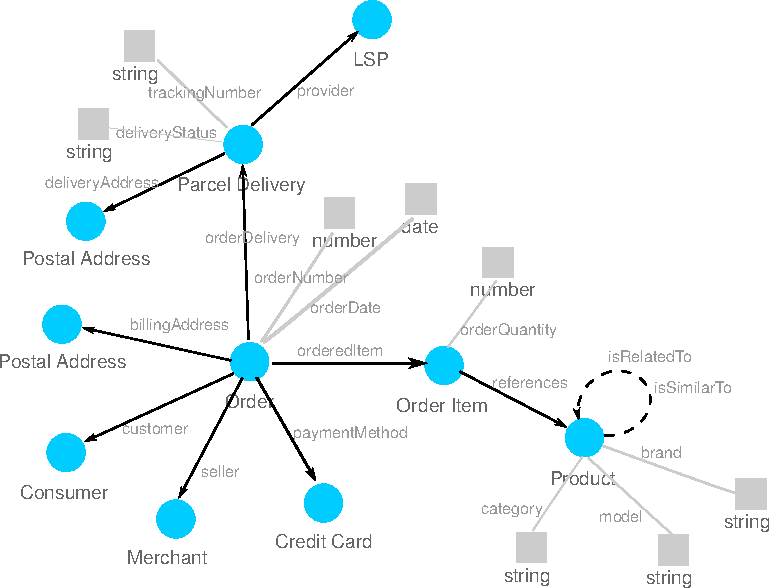
\includegraphics[width=0.8\columnwidth]{images/schema_org_mapping.pdf}
	\caption{Schema.org based mapping of the \gls{E-commerce} transaction}
\label{fig:images_schema_org}
\end{figure}

% subsec vocab_align

\subsection{Communication protocols}
\label{subsec:comm_protocol}

 The data is likely encoded in Microdata, \gls{RDFa} or \gls{JSON-LD}. \\

For the communication the \gls{WebRTC} is a good approach as it integrates well with existing enterprise IT infrastructures.

% subsec comm_protocol

\subsection{Partially centralized system architecture}
\label{subsec:p2p_partially_centralized_system}

The issuing bank is the trusted party in this system setup. It will initiate a data sharing session with the other required stakeholders based on the past usage of the credit card in question. During the P2P session the merchants, payment and logistic service providers will share the required information with the issuer. In this process the data from the other stakeholders will be replicated to the issuer, who will build up a graph based on the Schema.org schema mapping. The analysis of the data will be done on top of this graph by the issuer and can also be handled after the initial P2P data sharing session has been ended. If there are any new conclusions drawn from the data, the issuer is in charge to inform the stakeholders afterwards. So the main work will be on the issuer side, who is the major driving party in this scenario, as depicted in Figure~\ref{fig:images_p2p_centralized}.\@

\begin{figure}[H]
	\centering
		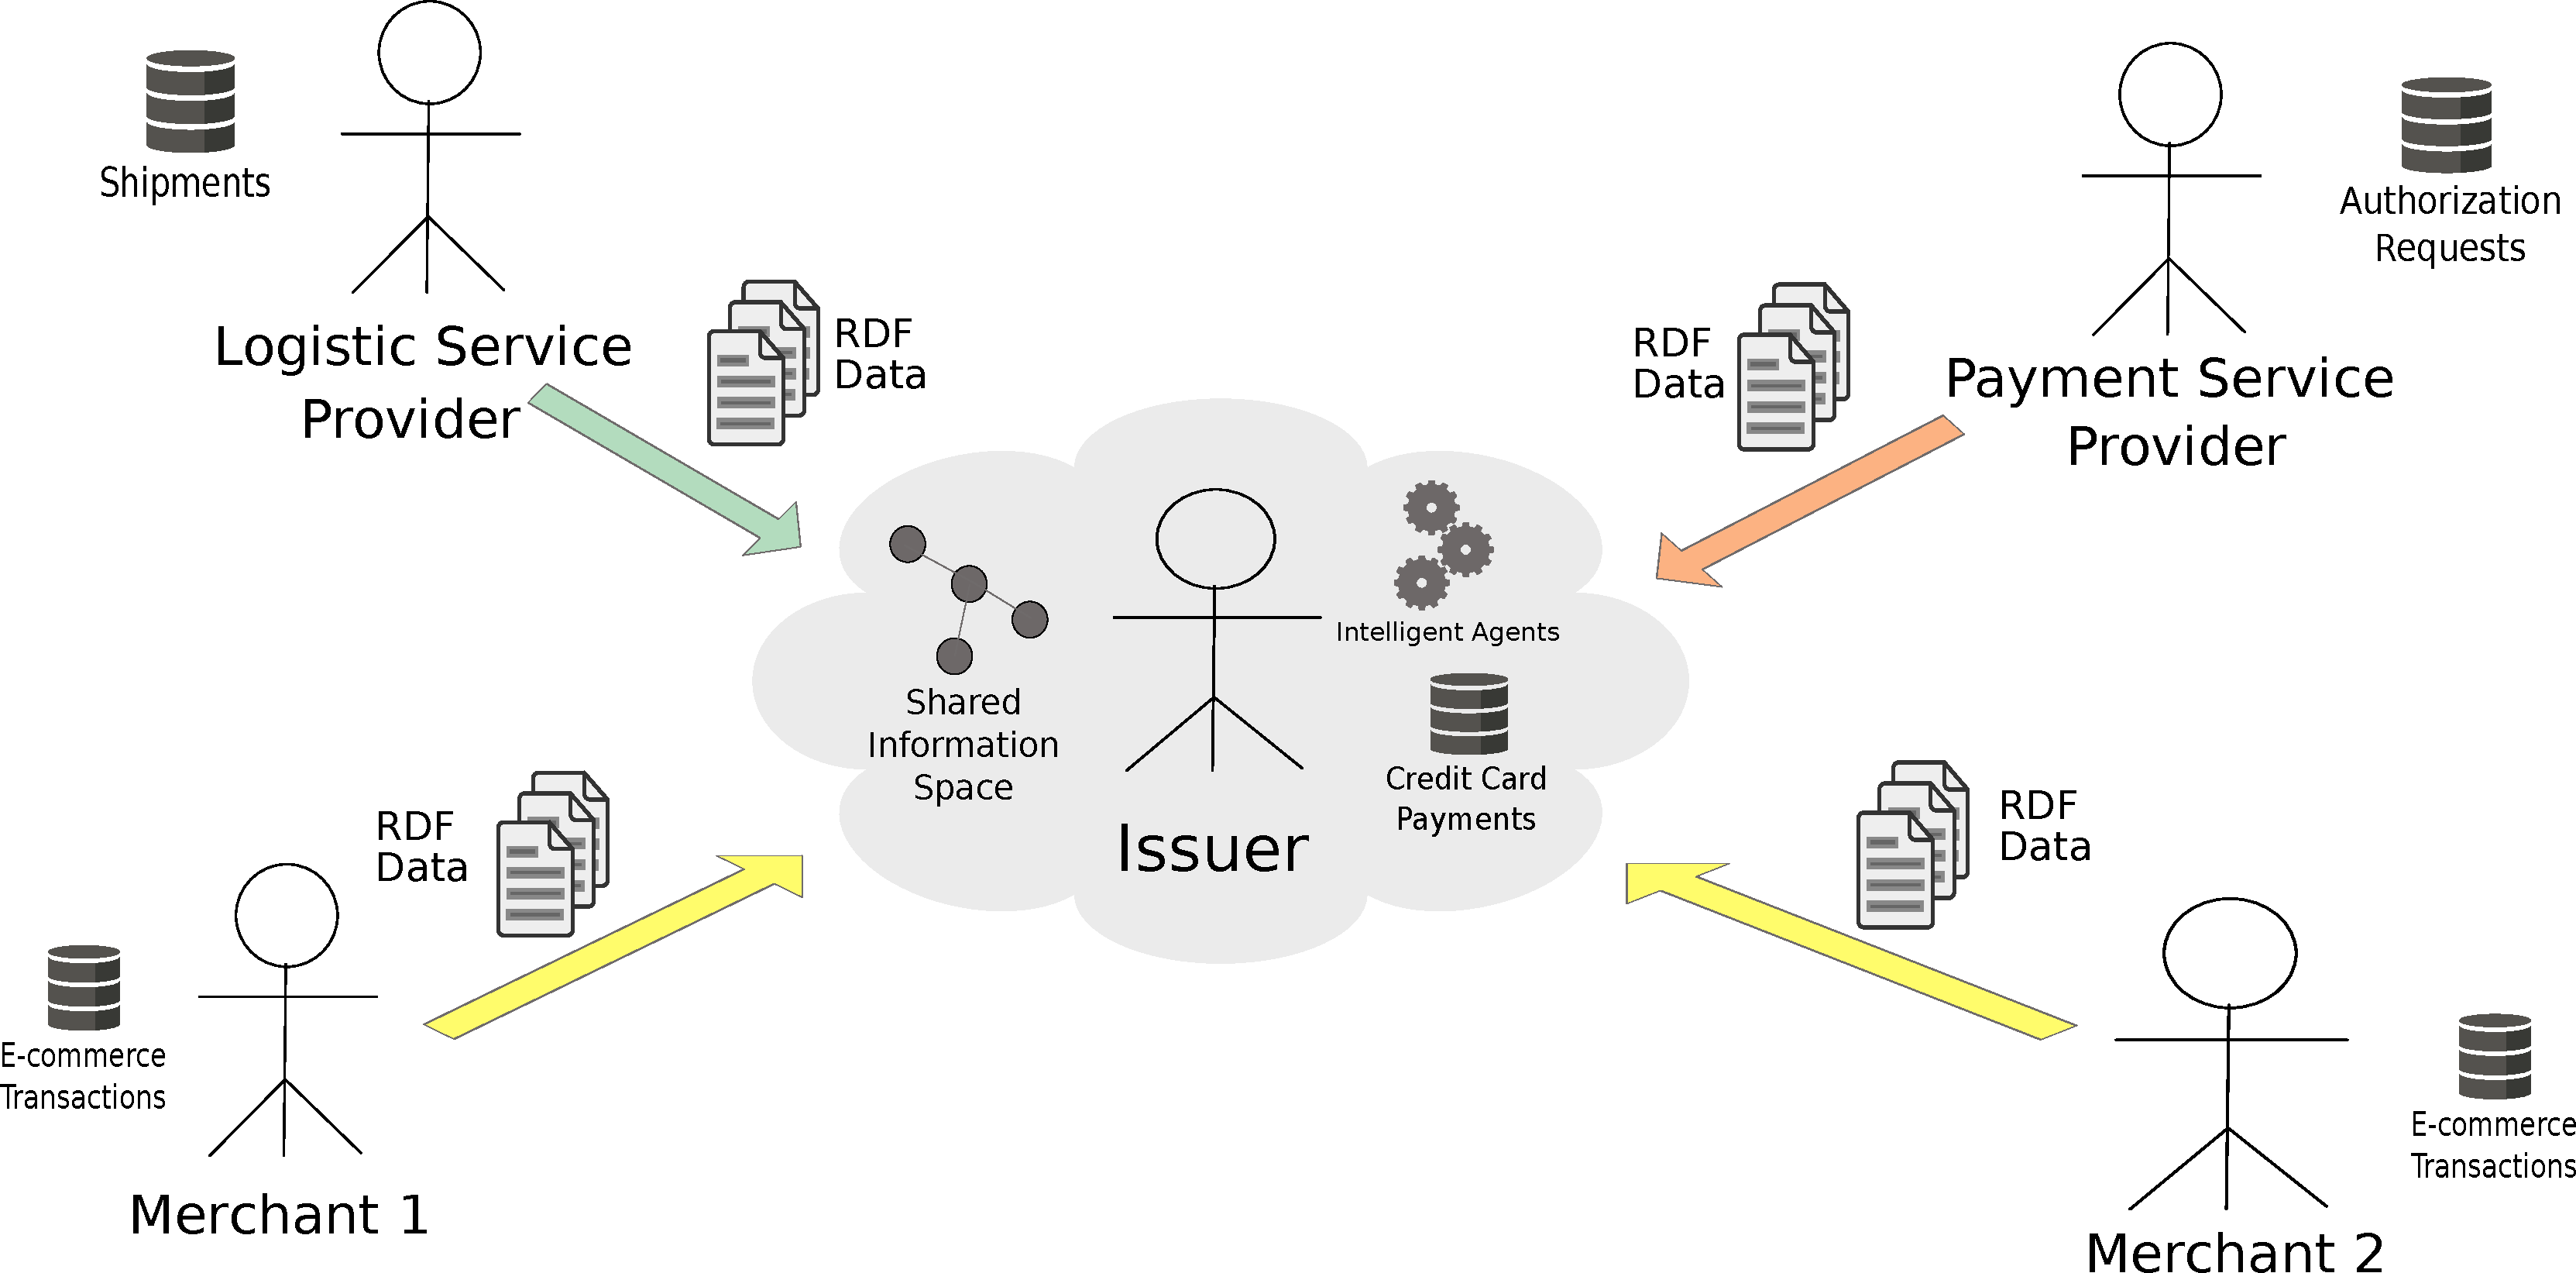
\includegraphics[width=0.8\columnwidth]{images/system_P2P_centralized.pdf}
	\caption{Partially centralized \gls{P2P} system architecture}
\label{fig:images_p2p_centralized}
\end{figure}

Main issue with the above mentioned system architecture is, that the merchants, payment and logistic service providers have to hand over their information to the issuing bank of the credit card for analysis. This might be either problematic due to distrust of the objectives of the issuing bank, or not possible at all due to local data sharing restrictions and regulations.

% subsec p2p_partially_centralized_system

% section design_proposal (end)
